%% fancy header & foot
\pagestyle{fancy}
\lhead{[ELEC-H-2001] Électricité\\ LABO \no 1B : Circuits réactifs en régime - Phaseurs et impédances \ifthenelse{\boolean{corrige}}{~-- corrigé}{}}
\rhead{v1.0.0\\ page \thepage}
\cfoot{}
%%
\usepackage{placeins}
\pdfinfo{
/Author (Renaud Theunissen et Youssef Agram, ULB -- BEAMS-EE)
/Title (Laboratoire 1B ELEC-H-2001, Circuits réactifs en régime - Phaseurs et impédances)
/ModDate (D:\pdfdate)
}

\hypersetup{
pdftitle={Labo 1A [ELEC-H-2001] Électricité : LABO 1B ELEC-H-2001, Circuits réactifs en régime - Phaseurs et impédances},
pdfauthor={Renaud Theunissen et Youssef Agram, ©2020 ULB - BEAMS-EE},
}


\setlength{\parskip}{0.5cm plus4mm minus3mm} %espacement entre §
\setlength{\parindent}{0pt}


\begin{document}

\tptitle{}{Séance 1B~: Circuits réactifs en régime - Phaseurs et impédances}
\section{But de la manipulation}
Le but de cette séance est de vous familiariser avec le matériel de laboratoire et à développer une approche d'investigation des phénomènes liés aux circuits électrique étudiés dans le cours d'ELEC-H-2001.

Pour ce laboratoire vous aurez besoin des éléments suivants :
\begin{itemize}
    \item Votre PicoScope
    \item Les trois sondes (câbles BNC fournit dans le kit).
    \item Le protoboard
    \item Les résistances $R_e$, $R_i$ et $R_j$
    \item L'inductance $L$
    \item Le condensateur $C_i$
\end{itemize}

\section{Pré-requis}
Pour réaliser cette séance de laboratoire, il vous est recommandé de relire attentivement les sections du syllabus suivantes :
\begin{itemize}
    \item Section 4.3 - Adaptation d'impédance
    \item Sections 5.1 à 5.3 - Loi des mailles et utilisation
    \item Section 7.3 - Phaseurs
    \item Section 7.4 - Impédances et admittances
\end{itemize}

\newpage

\subsection{Mesures de signaux et interprétation - circuit réactif \textbf{RL}}
Réalisez le circuit suivant sur votre \textit{Protoboard}:
\begin{center}
    \begin{circuitikz}\draw
        (0,0) to[sinusoidal voltage source, v=$v_G(t)$, i^>=$i(t)$] (0,4)
        to[resistor, l=$R_G$] (4,4)
        to[inductor, l_=$L$, v^<=$v_{charge}(t)$] (4,0) to[resistor, l=$R_e$] (0,0) node[ground]{};
    \end{circuitikz}
\end{center}
\Question{
En utilisant les outils du logiciel PicoScope 6:\\ 
\begin{enumerate}
    \item Utilisez un canal math pour représenter la tension $V_{charge}(t)$ à partir des signaux de tensions à la sortie du générateur et aux bornes de $R_e$.\\
    \textcolor{darkblue}{Le canal violet représente la tension aux bornes de l'inductance.
    \begin{figure}[h!]
        \centering
        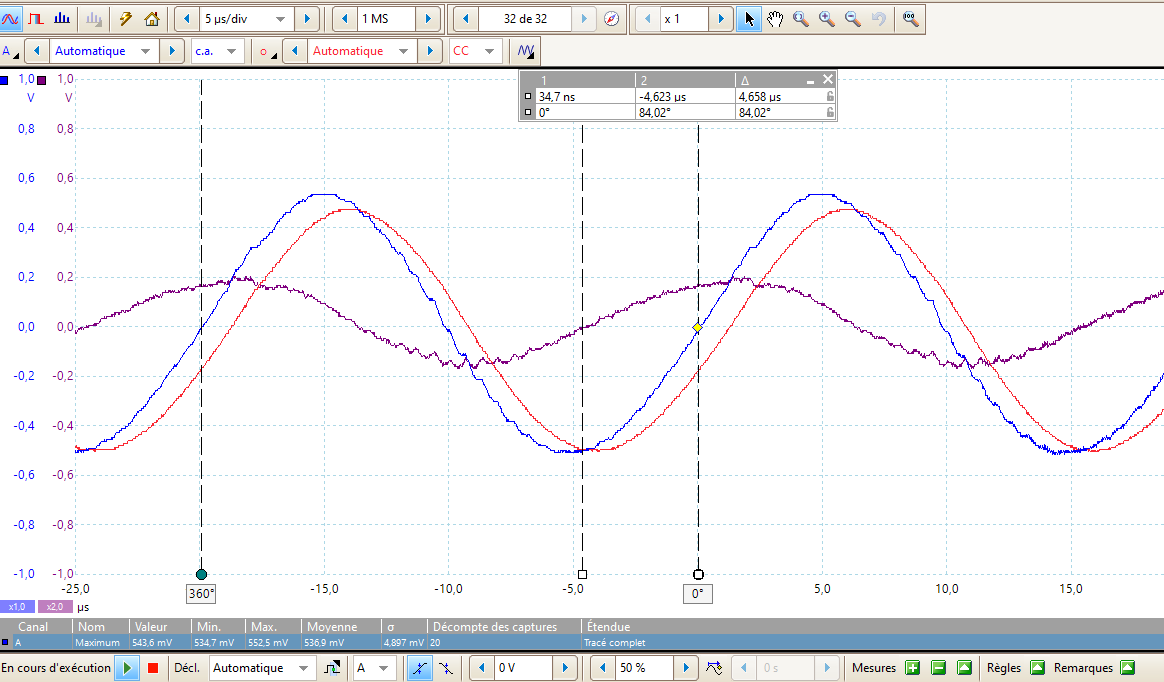
\includegraphics[scale=0.5]{TP2/RL_50k_R.png}
        \caption{Mesure de la tension aux bornes de l'inductance pour $f=50\ kHz$.}
        \label{fig:my_label}
    \end{figure}}
    \item Déterminez la plage de fréquences du signal $v_G(t)$ pour laquelle la tension $v_{charge}(t)$ est maximale.\\
    \textcolor{darkblue}{La transmittance du filtre étant $H(j\omega)=\frac{j\omega L}{R+j\omega L}$, le pole nous donne la fréquence de coupure du filtre: $p=-\frac{R_e}{L}=-909.1 \frac{krad}{s} \longrightarrow f_c=\frac{\omega}{2\pi}=144.7\ kHz$ . On est en présence d'un filtre \textbf{passe-haut}. L'oscilloscope présente un signal coupé aux alentours de 1 kHz et la tension sera maximale pour la plus grande valeur de fréquence i.e. 100 kHz.}
    \item Pour quelle fréquence le déphasage entre $v_G(t)$ et $v_{charge}(t)$ est-il le plus important?\\
    \\
    \FloatBarrier
    \begin{table}[h!]
        \centering
        \textcolor{darkblue}{
        \begin{tabular}{|c|c|c|c|}
        \hline
            & 10 kHz & 50 kHz & 100 kHz  \\
        \hline
        $\Delta \varphi$ & $84.47$°& $84$° & $68.57$°\\
        \hline
        \end{tabular}}
        \caption{Valeurs de déphasage pour différentes fréquences.}
        \label{tab:my_label}
    \end{table}
    \textcolor{darkblue}{Il devient ensuite difficile de mesurer le déphasage pour des fréquences inférieures. Par ailleurs, on devrait retrouver un déphasage de 45° à la fréquence de coupure.}
    \FloatBarrier
    \item Trouvez la valeur de $L$ à partir de la mesure de la tension $v_{charge}(t)$ et de $v_{R_e}(t)$.\\
    \textcolor{darkblue}{On peut trouver la valeur de l'inductance L sur base des amplitudes $V_{charge}$ et $V_{R_e}$ car cette dernière est à l'image du courant qui circule dans la maille:
    $$
     \left\{
                \begin{array}{r c l}
                  \underline{V}_{R_e} & = & R_e\,\underline{I}\\
                  \underline{V}_{charge} & = & j\omega L\,\underline{I}\\
                \end{array}
              \right. \longrightarrow  L=\frac{R_e}{\omega}\frac{V_c}{V_{R_e}}=\frac{200\times0.315}{2\pi\,50\times10^3\times 0.98}\simeq 204.62\ \mu H$$
    Cette méthode est beaucoup plus simple analytiquement qu'utiliser la formule du diviseur impédant.}
\end{enumerate}}
    

\subsection{Mesures de signaux et interprétation - circuit réactif \textbf{RC}}
Réalisez le circuit suivant sur votre \textit{Protoboard}:\\
\begin{center}
    \begin{circuitikz}\draw
        (0,0) to[sinusoidal voltage source, v=$v_G(t)$, i^>=$i(t)$] (0,4)
        to[resistor, l=$R_G$] (4,4)
        to[capacitor, l_=$C_i$, v^<=$v_{charge}(t)$] (4,0) to[resistor, l=$R_e$] (0,0) node[ground]{};
    \end{circuitikz}
\end{center}

En utilisant les outils du logiciel PicoScope 6: 
\Question{
\begin{enumerate}
    \item Utilisez un canal math pour représenter la tension $V_{charge}(t)$ à partir des signaux de tensions à la sortie du générateur et aux bornes de $R_e$.\\
   \begin{figure}[h!]
       \centering
       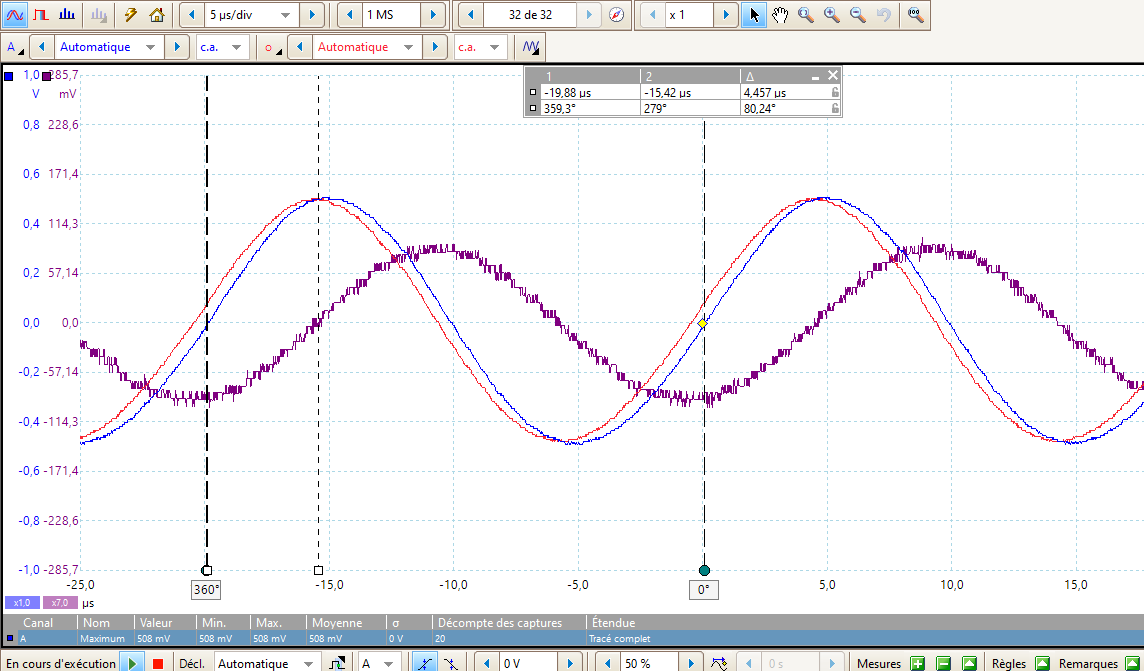
\includegraphics[scale=0.5]{TP2/RC_50k_R.png}
       \caption{Mesure de la tension aux bornes de la capacité pour $f=50\ kHz$.}
       \label{fig:my_label}
   \end{figure}
    \item Déterminez la plage de fréquences du signal $v_G(t)$ pour laquelle la tension $v_{charge}(t)$ est maximale.\\
     \textcolor{darkblue}{La transmittance du filtre étant $H(j\omega)=\frac{1}{1+j\omega RC}$, le pole nous donne la fréquence de coupure du filtre: $p=-\frac{1}{RC} \longrightarrow f_c=7.96\ kHz$ . On est en présence d'un filtre \textbf{passe-bas}. Malgré la fréquence de coupure atteinte, on distingue encore un signal à la fréquence max de la bande passante i.e. 100 kHz. L'amplitude semble être maximale sur la plage $[0\,Hz,100\,Hz]$.}
    \item Pour quelle fréquence le déphasage entre $v_G(t)$ et $v_{charge}(t)$ est-il le plus important?\\
    \FloatBarrier
    \begin{table}[h!]
        \centering
        \textcolor{darkblue}{
        \begin{tabular}{|c|c|c|c|c|c|}
        \hline
            & 100 Hz & 1 kHz & 10 kHz & 50 kHz & 100 kHz  \\
        \hline        $\Delta \varphi$ & $\simeq 0$°& $-8.09$° & $-48.46$° & $-78.95$° & $-85.52$°\\
        \hline
        \end{tabular}}
        \caption{Valeurs de déphasage pour différentes fréquences.}
        \label{tab:my_label}
    \end{table}
    \FloatBarrier
    \textcolor{darkblue}{Le déphasage devrait valoir -45° à la fréquence de coupure.}
    \item Trouvez la valeur de $C_i$ à partir de la mesure de la tension $v_{charge}(t)$ et de $v_{R_e}(t)$.
    \textcolor{darkblue}{On peut trouver la valeur de la capacité similairement:
    $$
     \left\{
                \begin{array}{r c l}
                  \underline{V}_{R_e} & = & R_e\,\underline{I}\\
                  \underline{V}_{charge} & = &\frac{1}{j\omega C}\,\underline{I}\\
                \end{array}
              \right. \longrightarrow  C=\frac{1}{\omega R}\frac{V_{R_e}}{V_{charge}}\simeq0.1 \,\micro F$$
    }
\end{enumerate}}{}

\subsection{Mesures de signaux et interprétation - circuit RLC}
Réalisez le circuit suivant :
\begin{center}
    \begin{circuitikz}\draw
    (0,0) to[sinusoidal voltage source, v=$v_G(t)$, i^>=$i_G(t)$] 
    (0,4)   to[resistor, l=$R_G$] 
    (4,4)   to[inductor, l=$L$] (4,0)
    (4,4)--(6,4)   to[capacitor, l_=$C_i$, v^<=$v_{charge}(t)$]
    (6,0)--(4,0) to[resistor, l=$R_e$] (0,0)   node[ground]{}
    ;
    \end{circuitikz}
\end{center}
Réglez la source de tension avec une amplitude de $V_m=2V$ et une fréquence de $50 kHz$.
\Question{
\begin{enumerate}
    \item Déterminez une plage de fréquence pour laquelle la tension $v_{charge}$ à une amplitude supérieure à la tension $v_{R_e}$.\\
    \textcolor{darkblue}{Nous sommes en présence d'un filtre d'ordre 2. En effet, nous pouvons calculer la fonction de transfert du circuit avec $\underline{V}_{in}$. Il ne faut pas prendre en compte la résistance $R_G$ dans le filtre car les signaux sont mesurés en sortie du générateur. 
    $$
     \left\{
                \begin{array}{r c l}
                  Z_{eq} & = & \frac{Z_L\,Z_C}{Z_L+Z_C}\\
                  \underline{V}_{charge} & = &\frac{Z_{eq}}{Z_{eq}+R_e}\,\underline{V}_{in}\\
                \end{array}
              \right. \longrightarrow H(p)=\frac{pL}{R_e\,(1+p^2LC)+pL}$$ 
              $$H(p)=\frac{pL}{R_eLC\,p^2+Lp+R_e}$$\\
    On a donc 1 zéro à l'origine et 2 pôles complexes conjugués: $p_{1,2}=-\sigma \pm j\omega_d=(-25+j\,211.7)\times 10^3$. La fréquence de résonance vaut donc en principe $\omega_n=\sqrt{\sigma^2+\omega_d^2}=213.171\ kHz$. On a donc un pic de résonance autour de cette fréquence avec une atténuation aux basses et hautes fréquences (filtre passe-bande).\\
    Sur le picoscope, on voit }
              
    \item Que devient l'amplitude de $v_{charge}$ pour une fréquence $f=500Hz$? Justifiez physiquement ce résultat.
    \item Donnez une plage de fréquence pour laquelle le déphasage entre $v_{charge}$ et $v_{R_e}$ est maximal.
\end{enumerate}}{}

\end{document}